\documentclass[sn-mathphys-num]{sn-jnl}
\usepackage{amssymb}
%% The amsmath package provides various useful equation environments.
% In preamble

\usepackage{amsmath}
\usepackage{soul}
\usepackage{xcolor}
\usepackage{cancel}
\usepackage{enumitem}
\usepackage{tcolorbox}
\usepackage{afterpage}
\usepackage{float}


% Math and logic
\usepackage{amssymb}
\usepackage{amsmath}
\usepackage{array}
\usepackage{multirow}
\usepackage{ragged2e}
\usepackage{booktabs}


% Tables and figures
\usepackage{tabularx}
\usepackage{longtable}
\usepackage{rotating}
\usepackage{graphicx}
\usepackage{subcaption}
\usepackage{hhline}

% Preamble
\usepackage{fontspec}
\newfontfamily\arabicfont[Script=Arabic]{Amiri}

\newcommand{\RTL}[1]{%
  \bgroup
  \arabicfont
  \textdir TRT\pardir TRT
  #1%
  \egroup
}

\usepackage{lineno}
\linenumbers

\begin{document}

\title[Arabic News Classification: Lightweight Supervised Models vs. Zero-Shot Large Language Models]{Arabic News Classification: Lightweight Supervised Models vs. Zero-Shot Large Language Models}

\author[1]{\fnm{Omar} \sur{Elgendy}}\email{oelgendy@sharjah.ac.ae}
\author[1]{\fnm{Ali} \sur{Bou Nassif}}\email{anassif@sharjah.ac.ae}
\author*[2]{\fnm{Ashraf} \sur{Elnagar}}\email{ashraf@sharjah.ac.ae}
% \equalcont{Corresponding author.}

\affil[1]{\orgdiv{Department of Computer Engineering}, \orgname{University of Sharjah}, \state{Sharjah}, \country{UAE}}
\affil[2]{\orgdiv{Department of Computer Science}, \orgname{University of Sharjah}, \state{Sharjah}, \country{UAE}}

\abstract{
 This paper presents a comparative analysis of lightweight supervised models and zero-shot large language models (LLMs) for Arabic text classification. We use the AlKhaleej subset of the SANAD dataset, a clean and balanced corpus classifying seven news categories. For the supervised models, we leverage CAMeLBERT pre-trained embeddings with two classification heads: a dense neural layer and a linear SVM. For the LLMs, we evaluate four state-of-the-art zero-shot models: GPT-4.1, DeepSeek V3, Gemini 2.0-Flash, and Claude 3.5-Haiku, using a unified prompt-based setup. Results show that the fine-tuned supervised models consistently outperform the zero-shot LLMs, with the dense-head model achieving 97\% accuracy compared to 93\% from the best-performing LLM. The SVM model trains 58\% faster, while the dense model offers slightly faster inference. Category-wise analysis reveals that supervised models maintain robust performance across all classes, whereas zero-shot LLMs exhibit notable degradation in semantically sensitive categories such as religion. These findings highlight the continued advantage of domain-adapted models for Arabic classification tasks and suggest promising directions for hybrid approaches that combine task-specific tuning with the generalization strengths of LLMs.
}

\keywords{Arabic NLP, Multi-label Classification, text classification, light-weight models, LLMs}

\maketitle


\section{Introduction}
\label{intro}

Text classification constitutes a fundamental task within natural language processing, underpinning diverse applications ranging from sentiment analysis \cite{elnagar2021sentiment,bensoltane2022towards,bentrcia2025hybrid}  to fake news detection \cite{nassif2022arabic} and hate speech filtering \cite{elgendy2024toxicity, torfa2025enhancing}. Despite substantial progress driven by deep learning methods—most notably transformer-based architectures—significant obstacles persist when dealing with morphologically complex and low-resource languages, Arabic being a prominent example. The language presents particular challenges stemming from its intricate script system, considerable orthographic variability, and elaborate morphological structure, all of which are further complicated by the coexistence of more than twenty regional dialects \cite{helwe2020semi, talafha2020multi}. Although transformer models have advanced the state of Arabic NLP, progress in this domain continues to follow that observed for English and other well-resourced languages, a gap attributable primarily to the scarcity of annotated data, pronounced domain-specific variation, and class imbalance within available datasets \cite{alhawarat2020superior, almuzaini2020impact}. Such constraints prove particularly acute in scenarios where computational resources are limited or rapid deployment is required, rendering large-scale models impractical.

The Transformer architecture \cite{vaswani2017attention} has given rise to a succession of influential models, including BERT \cite{devlin2018bert}, T5 \cite{roberts2019exploring}, GPT \cite{DBLP:journals/corr/abs-2005-14165}, LLaMA \cite{touvron2023llama}, and Falcon \cite{almazrouei2023falcon}. These systems exhibit robust generalization abilities, performing well even under zero-shot conditions as shown in \cite{DBLP:journals/corr/abs-1909-00161} and \cite{gera2022zero}, and have demonstrated considerable language understanding across varied tasks. Nonetheless, their performance on specific Arabic NLP problems—multi-class news classification among them—has received comparatively little attention \cite{wahdan2024systematic}. Evidence from existing research suggests that models fine-tuned for particular tasks frequently surpass general-purpose large language models in terms of both classification accuracy and computational efficiency when processing Arabic text \cite{alruily2023automated, nassif2022arabic}. Yet systematic comparisons between these two paradigms within the Arabic domain remain scarce.

This study aims to address that gap through a systematic comparison of two lightweight supervised models—built using CAMeLBERT embeddings—against leading zero-shot LLMs, including GPT-4.1, DeepSeek, Claude, and Gemini for Arabic Text Classification. We conduct our evaluation on the balanced AlKhaleej subset of the SANAD dataset, which comprises seven news categories: \textit{Culture}, \textit{Finance}, \textit{Medical}, \textit{Politics}, \textit{Religion}, \textit{Sports}, and \textit{Tech}. In addition to classification accuracy, we assess runtime performance during training and inference, with the goal of understanding the trade-offs between accuracy, efficiency, and deployment feasibility.

This work offers three principal contributions:
\begin{itemize}
    \item We introduce and evaluate two lightweight classification architectures that leverage CAMeLBERT embeddings coupled with either a dense neural network classifier or a linear support vector machine.
    \item We systematically benchmark these models against contemporary zero-shot large language models, employing a unified prompt-based evaluation protocol to guarantee fair and consistent comparison across all systems.
    \item We provide a detailed analysis of classification performance at the category level alongside an assessment of both training and inference efficiency, yielding practical guidance for model selection in real-world Arabic NLP deployments.
\end{itemize}

This study highlights when and why fine-tuned models continue to outperform general-purpose LLMs in Arabic classification tasks, while also identifying scenarios where zero-shot systems perform competitively or fall short. Our findings aim to support both researchers and practitioners in choosing models that balance accuracy, efficiency, and scalability for Arabic-language NLP.
As the field increasingly explores the trade-offs between task-specific fine-tuning and general-purpose modeling, our work contributes timely empirical evidence from a low-resource, morphologically complex language that remains underrepresented in current zero-shot evaluations.

The remainder of this paper proceeds as follows. Section~\ref{rel-works} surveys prior work on Arabic text classification and examines the application of large language models under zero-shot conditions. Section~\ref{methodology} details our methodology, encompassing the dataset, model architectures, prompt design, hyperparameter settings, and computational infrastructure. Section~\ref{results} reports the experimental findings and accompanying analysis. Section~\ref{discussion} interprets the principal results, considers their practical implications, and acknowledges the limitations of our study. Section~\ref{conclusion} concludes with a summary of contributions and prospective directions for future research.

\section{Related Work}
\label{rel-works}

\subsection{Arabic Text Classification}
Arabic text classification has received growing attention due to the Arabic language morphological richness and dialectal diversity. Early efforts relied on traditional machine learning with TF-IDF and n-grams \cite{omar2021multi}. More recent work applied deep neural architectures such as CNNs and RNNs, achieving strong results on news and social media datasets \cite{muaad2022effective,almuzaini2020impact}. For example, SATCDM, a multi-kernel CNN, reached accuracies above 97\% on several benchmarks \cite{alhawarat2020superior}. Despite these gains, traditional neural models remain limited by their dependence on handcrafted features, long training times, and poor cross-dialect generalization.

The release of large Arabic corpora such as SANAD \cite{elnagar2020arabic} enabled systematic evaluation across multiple categories. Models trained on this dataset, including BiGRU and CLSTM, exceeded 96\% accuracy. However, most studies evaluated only deep supervised setups, often under single-label assumptions, without testing emerging large language models \cite{rifai2021arabic,el2022arabic}.

\subsection{Arabic Transformer Models}
The introduction of Arabic-specific transformer models marked a turning point in Arabic NLP. AraBERT \cite{helwe2020semi} demonstrated that domain-adapted pretraining on Arabic corpora outperformed multilingual BERT across sentiment, NER, and dialect identification tasks. Successive models such as MARBERT, ARBERT, and QARiB extended coverage to dialectal Arabic. CAMeLBERT, trained on a large clean corpus, showed strong performance on classification and morphological tasks and became a reliable baseline for downstream Arabic applications \cite{yagi2021evaluation,elnagar2023benchmark,nassif2022arabic}.

Benchmarks confirm the importance of Arabic-specific transformers. Nassif et al. \cite{nassif2022arabic} evaluated multiple Arabic and multilingual models on fake news detection. Results showed ARBERT and QARiB outperforming translated datasets and multilingual baselines, reaching up to 98.8\% accuracy. Elgendy et al. \cite{elgendy2024toxicity} extended this line by analyzing bias detection in Arabic texts, highlighting the importance of domain-specific evaluation. These studies emphasize that high-quality pretraining and native datasets remain essential for robust Arabic classification.

\subsection{Few-Shot and Zero-Shot LLMs}
The rise of large language models (LLMs) such as GPT-3, GPT-4, Claude, Gemini, and DeepSeek introduced the possibility of zero-shot and few-shot learning for Arabic tasks. While multilingual LLMs exhibit strong performance in high-resource languages, their results in Arabic are inconsistent. For example, Zhang and Abdul-Mageed \cite{zhang2019bert} showed that multilingual BERT improves author attribute prediction on Arabic tweets, but dialect classification accuracy remained modest. More broadly, recent evaluations of LLMs on Arabic benchmarks confirm that while they provide competitive results without task-specific training, they still underperform fine-tuned Arabic models in domain-sensitive settings \cite{baniata2023transformer,hossain2024transnet}.

Studies outside Arabic also confirm this trend. Bao et al. \cite{bao2019few} showed that few-shot methods improve classification under limited supervision, but require high-quality prompts and unlabeled data. Comparative works in other low-resource languages reveal that fine-tuned lightweight transformers remain superior to zero-shot LLMs in accuracy and efficiency \cite{ali2022deep}.

\sloppy
\subsection{Evaluation and Research Gap}
Existing Arabic benchmarks highlight the performance of supervised models \cite{nassif2022arabic, elgendy2024toxicity}, while recent work has tested LLMs in limited zero-shot contexts. However, no prior study has systematically compared fine-tuned lightweight Arabic transformers such as CAMeLBERT against modern zero-shot LLMs on the same multi-class classification dataset. Moreover, efficiency metrics such as training time, inference speed, and robustness across categories remain underexplored. Our work addresses this gap by directly benchmarking lightweight supervised models against GPT-4.1, Claude 3.5-Haiku, Gemini 2.0-Flash, and DeepSeek V3, offering both performance and efficiency comparisons on the SANAD-AlKhaleej corpus.

\section{Methodology}
\label{methodology}
\label{dataset}
\subsection{Dataset}

This work utilizes the \textbf{SANAD (Single-Label Arabic News Articles Dataset)} introduced by Einea et al.~\cite{elnagar2020arabic}, a large-scale labeled corpus designed to support Arabic natural language processing tasks such as text classification, document clustering, and word embedding learning. The dataset was compiled using automated scripts that collected articles from three major Arabic news outlets: \textit{AlKhaleej}, \textit{AlArabiya}, and \textit{Akhbarona}. SANAD contains more than 190,000 articles categorized into seven distinct topics: \textit{Culture}, \textit{Finance}, \textit{Medical}, \textit{Politics}, \textit{Religion}, \textit{Sports}, and \textit{Tech}. The only exception is the \textit{AlArabiya} subset, which excludes the \textit{Religion} category due to source limitations. The text is written in Modern Standard Arabic and follows the formal style of journalistic reporting. This work focuses on the AlKhaleej subset, which includes {45,500 articles}, equally distributed among the seven categories. Each article is labeled with a single class, making the dataset well-suited for multi-class classification tasks. The SANAD dataset has several key characteristics that make it suitable for supervised learning tasks. The AlKhaleej subset maintains a uniform label distribution, allowing for fair evaluation across different categories. The text is clean and written in formal Modern Standard Arabic, which ensures consistency and clarity. Additionally, the dataset covers a wide range of news topics, providing diverse language use and content that reflect real-world scenarios.

\vspace{0.3cm}
To visualize the dataset structure, Figure ~\ref{fig:category_percent} presents a pie chart illustrating the percentage distribution of articles across categories, with each category accounting for approximately 14.3\% as shown below, confirming the balanced nature of the dataset.

\vspace{0.6cm}
\begin{figure}[!ht]
    \centering
        \centering
        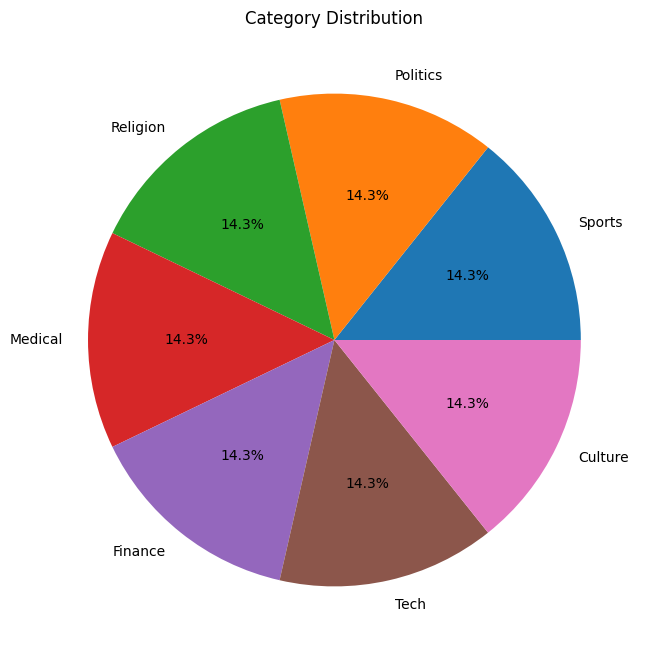
\includegraphics[width=0.7\textwidth]{data categories dist perc.png}
        \caption{Percentage Distribution of Articles per Category}
        \label{fig:category_percent}
    \hfill
    \caption{Visual analysis of SANAD (AlKhaleej subset) category distribution.}
    \label{fig:category_analysis}
\end{figure}

To ensure fair and consistent model evaluation, the dataset was split into three subsets: \textbf{training}, \textbf{validation}, and \textbf{testing}. The splitting was performed using stratified sampling to maintain the original category distribution across all subsets. This prevents category imbalance in any subset, which could otherwise bias the training or evaluation process. The split ratios are as follows:
\begin{itemize}
    \item 70\% for training (\textasciitilde31,850 articles)
    \item 15\% for validation (\textasciitilde6,825 articles)
    \item 15\% for testing (\textasciitilde6,825 articles)
\end{itemize}

\subsection{Models}

This study implements and compares three classifier systems for Arabic text classification, evaluating their performance across accuracy, precision, recall, F1-score, and, where applicable, training and inference time.

Two models rely on CAMeLBERT for Modern Standard Arabic \cite{DBLP:journals/corr/abs-2103-06678}, used as a frozen feature extractor that generates 768-dimensional contextual embeddings. The first model, \textbf{BERT–Dense}, integrates these embeddings with a lightweight neural classifier. The second model, \textbf{BERT–SVM}, applies a Support Vector Machine (SVM) using a radial basis function (RBF) kernel. The third approach employs \textbf{zero-shot inference} from large language models (LLMs) accessed through public APIs.

\noindent The architecture of the BERT–Dense model is defined as:
\begin{itemize}
    \item \textbf{Input:} 768-dimensional CAMeLBERT embeddings.
    \item \textbf{Layer 1:} Fully connected linear layer (768 $\rightarrow$ 384 units) with ReLU activation.
    \item \textbf{Layer 2:} Dropout (probability = 0.25).
    \item \textbf{Layer 3:} Fully connected linear layer (384 $\rightarrow$ number of classes).
    \item \textbf{Output:} Logit scores across seven target categories.
\end{itemize}

\noindent The BERT–SVM configuration is as follows:
\begin{itemize}
    \item \textbf{Kernel:} Radial Basis Function (RBF)
    \item \textbf{Degree:} 6
    \item \textbf{Gamma:} \texttt{scale}
    \item \textbf{Regularization (C):} 9
\end{itemize}

\sloppy
\noindent
CAMeLBERT was intentionally used as a frozen encoder rather than being fine-tuned for three main reasons:
\begin{itemize}
    \item Domain-specific Arabic labeled data are scarce, and prior benchmark studies have shown that frozen contextualized embeddings often provide more stable generalization under limited supervision \cite{AlAyyoub2017, antoun2020,elnagar2023benchmark}.
    \item Freezing transformer layers preserves linguistic generalization from large Arabic corpora, ensuring consistent embeddings across experiments.
    \item Freezing the encoder reduces computational cost, improving reproducibility and suitability for low-resource environments.
\end{itemize}

\sloppy
\noindent
This setup isolates the effect of classifier architecture on task performance rather than representation quality, aligning with established transfer learning practices in resource-constrained scenarios. The three systems represent distinct learning paradigms. The \textbf{BERT–SVM} is non-parametric, relying on geometric separation within the embedding space. The \textbf{BERT–Dense} introduces limited trainable capacity to adapt to semantic nuances. The \textbf{Zero-Shot LLMs} instead use implicit reasoning from large-scale linguistic priors, enabling context-based prediction without explicit training. Table~\ref{tab:models_summary} summarizes the model configurations.

\begin{table}[!ht]
\centering
\caption{Summary of the classification models used in this study}
\label{tab:models_summary}
\small
\begin{tabular}{@{}>{\raggedright\arraybackslash}p{3.5cm} >{\raggedright\arraybackslash}p{8cm}@{}}
\hline
\textbf{Model Name} & \textbf{Description} \\
\hline
BERT–Dense Head & CAMeLBERT-MSA (\texttt{bert-base-arabic-camelbert-msa}) as a frozen encoder. Classifier: Linear–Dropout–Linear. Only dense layers are trainable. Designed for efficient task adaptation. \\
BERT–SVM (RBF) Head & CAMeLBERT-MSA embeddings classified using an SVM with RBF kernel (degree 6, gamma = \texttt{scale}, C = 9). A geometric classifier relying solely on feature space separability. \\
Zero-Shot LLMs & GPT-4.1, Claude 3.5-Haiku, Gemini 2.0-Flash, and DeepSeek V3 accessed via API using a unified Arabic prompt. Predictions are made without fine-tuning. Inference time is excluded due to external variability. \\
\hline
\end{tabular}
\end{table}

\noindent
LLM-generated responses were post-processed through a rule-based mapping to align model outputs with the seven target categories. We mentioned explicitly in the system prompt that the output must be only one word corresponds to that class. We will discuss this deeper in the next subsection Prompt Engineering. 

This additional step highlights a key limitation of zero-shot inference: despite robust linguistic reasoning, generative variability introduces label inconsistency, especially in morphologically rich or culturally specific contexts. In contrast, supervised classifiers maintain deterministic label output once trained.

Overall, the comparative analysis of frozen BERT-based classifiers and zero-shot LLMs enables a controlled exploration of accuracy–efficiency trade-offs and the practical viability of LLM-based inference in Arabic NLP.

\subsection{Prompt Engineering}

To evaluate the zero-shot classification capabilities of large language models (LLMs) on Arabic text, a unified prompt format was applied across all tested models. This ensured consistent task framing and eliminated confounding factors during comparison. The prompt was structured as follows:

\begin{quote}
\textit{You are an Arabic text classifier. Classify the following sentence into one of the categories below:\\
\texttt{[List of categories]}\\
Sentence: \texttt{[Input text]}\\
Class:}
\end{quote}

This design followed four key principles:
\begin{itemize}
    \item Instruction clarity: Clearly defines the model\'s role as a classifier.
    \item Label grounding: Embeds all possible categories to constrain output.
    \item Input specificity: Focuses the prompt on a single sentence.
    \item Output constraint: Instructs the model to return only the predicted class label.
\end{itemize}

No few-shot examples or system messages were included to maintain a true zero-shot setting. All four LLMs—GPT-4.1, Claude 3.5-Haiku, Gemini 2.0-Flash, and DeepSeek V3—received identical prompts to ensure fairness. Model outputs were post-processed using exact or partial string matching to map predictions to the predefined class labels.

The significant variation in performance observed among the LLMs underscores a critical dependency on prompt sensitivity and training data coverage. Zero-shot prompts are notably brittle; their effectiveness can vary drastically with minor wording changes, especially when dealing with semantically rich or overlapping categories. Unlike supervised models fine-tuned for structured outputs, general-purpose LLMs are not explicitly optimized for classification tasks, which can lead to inconsistencies in category mapping and formatting. For instance, Claude 3.5-Haiku\'s poor performance on categories such as \textit{Religion} may reflect either limited exposure to culturally specific Arabic concepts in its training data or difficulties in grounding the classification task without additional contextual priming from the prompt.

\subsection{Hyperparameters and Training Configuration}

To ensure reproducibility, we report all hyperparameters used for training the BERT-based classification models. Table~\ref{tab:hyperparameters} summarizes the complete training configuration for both the BERT–Dense and BERT–SVM models.

\begin{table}[!ht]
\centering
\caption{Hyperparameter configuration for BERT-based models}
\label{tab:hyperparameters}
\small
\begin{tabular}{l l l}
\hline
\textbf{Hyperparameter} & \textbf{BERT–Dense} & \textbf{BERT–SVM} \\
\hline
Base Model & CAMeLBERT-MSA & CAMeLBERT-MSA \\
Embedding Dimension & 768 & 768 \\
Encoder State & Frozen & Frozen \\
\hline
\multicolumn{3}{l}{\textit{Classifier-Specific Parameters}} \\
\hline
Optimizer & AdamW & N/A \\
Learning Rate & $5 \times 10^{-5}$ & N/A \\
Epochs & 10 & N/A \\
Batch Size & 32 & 32 (embedding extraction) \\
Loss Function & CrossEntropyLoss & N/A \\
Dropout Rate & 0.25 & N/A \\
Hidden Layer Size & 384 & N/A \\
SVM Kernel & N/A & RBF \\
SVM Degree & N/A & 6 \\
SVM Gamma & N/A & \texttt{scale} \\
SVM Regularization (C) & N/A & 9 \\
\hline
\multicolumn{3}{l}{\textit{Reproducibility}} \\
\hline
Random Seed & 42 & 42 \\
\hline
\end{tabular}
\end{table}

\noindent
The random seed was fixed across Python \texttt{random} module, NumPy, PyTorch, and the Transformers library to ensure deterministic behavior. For the BERT–Dense model, the AdamW optimizer was chosen for its effective handling of weight decay regularization, which helps prevent overfitting in the classification head. The learning rate of $5*10^{-5}$ follows established best practices for training lightweight heads in frozen transformer encodings. Training was conducted for 10 epochs with early stopping based on validation loss to prevent overfitting. For the BERT–SVM model, embeddings were extracted in batches of 32 samples, and the SVM was trained on the complete set of pre-computed embeddings using GPU-accelerated implementation via cuML.

\subsection{Infrastructure}
All experiments were conducted on an NVIDIA A100 GPU with 40GB of VRAM, hosted on a cloud computing platform (vast.ai). The software environment consisted of Python 3.10, PyTorch 2.0 with CUDA 11.8, and the Hugging Face Transformers library (version 4.48). For the BERT–SVM model, GPU-accelerated SVM training was enabled using RAPIDS cuML, which significantly reduced training time compared to CPU-based implementations. Table~\ref{tab:infrastructure} provides a detailed summary of the experimental infrastructure.

\begin{table}[!ht]
\centering
\caption{Experimental infrastructure and software configuration}
\label{tab:infrastructure}
\small
\begin{tabular}{lcccc}
\hline
\textbf{Component} & \textbf{Specification} \\
\hline
GPU & NVIDIA A100 (40GB VRAM) \\
CUDA Version & 11.8 \\
Python Version & 3.10 \\
PyTorch Version & 2.0 \\
Transformers Library & 4.48 \\
cuML (RAPIDS) & GPU-accelerated SVM implementation \\
Experiment Tracking & Weights \& Biases (wandb) \\
\hline
\end{tabular}
\end{table}

\section{Experimental Results}
\label{results}

This section evaluates all models across accuracy, precision, recall, F1-score, training time, and inference time. Fine-tuned BERT architectures (Dense and SVM heads) are systematically compared against state-of-the-art zero-shot large language models (LLMs), including GPT-4.1, DeepSeek V3, Gemini-2.0-Flash, and Claude-3.5-Haiku. Both quantitative results and qualitative error analyses are reported to highlight model strengths, limitations, and practical deployment considerations.

Table~\ref{tab:all_models} presents the macro-averaged metrics. The fine-tuned CAMeLBERT variants reached 97\% accuracy with balanced precision and recall, clearly outperforming the zero-shot LLMs. Among external LLMs, GPT-4.1 and DeepSeek V3 achieved competitive results (93\%), followed by Gemini-2.0-Flash (91\%). Claude-3.5-Haiku lagged substantially, reaching only 75\% accuracy, with marked precision drops.

\begin{table}[!ht]
\centering
\caption{Comprehensive Model Performance Comparison (Macro-Averaged Metrics)}
\label{tab:all_models}
\small
\begin{tabular}{lcccc}
\hline
\textbf{Model} & \textbf{Accuracy} & \textbf{Precision} & \textbf{Recall} & \textbf{F1-score} \\
\hline
BERT Dense Head & 0.97 & 0.97 & 0.97 & 0.97 \\
BERT SVM Head & 0.97 & 0.97 & 0.97 & 0.97 \\
GPT-4.1 & 0.93 & 0.93 & 0.93 & 0.93 \\
DeepSeek V3 & 0.93 & 0.93 & 0.93 & 0.92 \\
Gemini-2.0-Flash & 0.91 & 0.92 & 0.91 & 0.91 \\
Claude-3.5-Haiku & 0.75 & 0.64 & 0.75 & 0.69 \\
\hline
\end{tabular}
\end{table}

\subsection{Class-Level Performance Analysis}

To understand the nuanced behavior of fine-tuned BERT models and explain why general-purpose LLMs underperform in certain categories, we present detailed per-class confusion matrices. Figures~\ref{fig:cm_dense_overall} and~\ref{fig:cm_svm_overall} show the overall confusion matrices for both BERT architectures, revealing patterns of misclassifications across all seven news categories.

\begin{figure}[!ht]
\centering
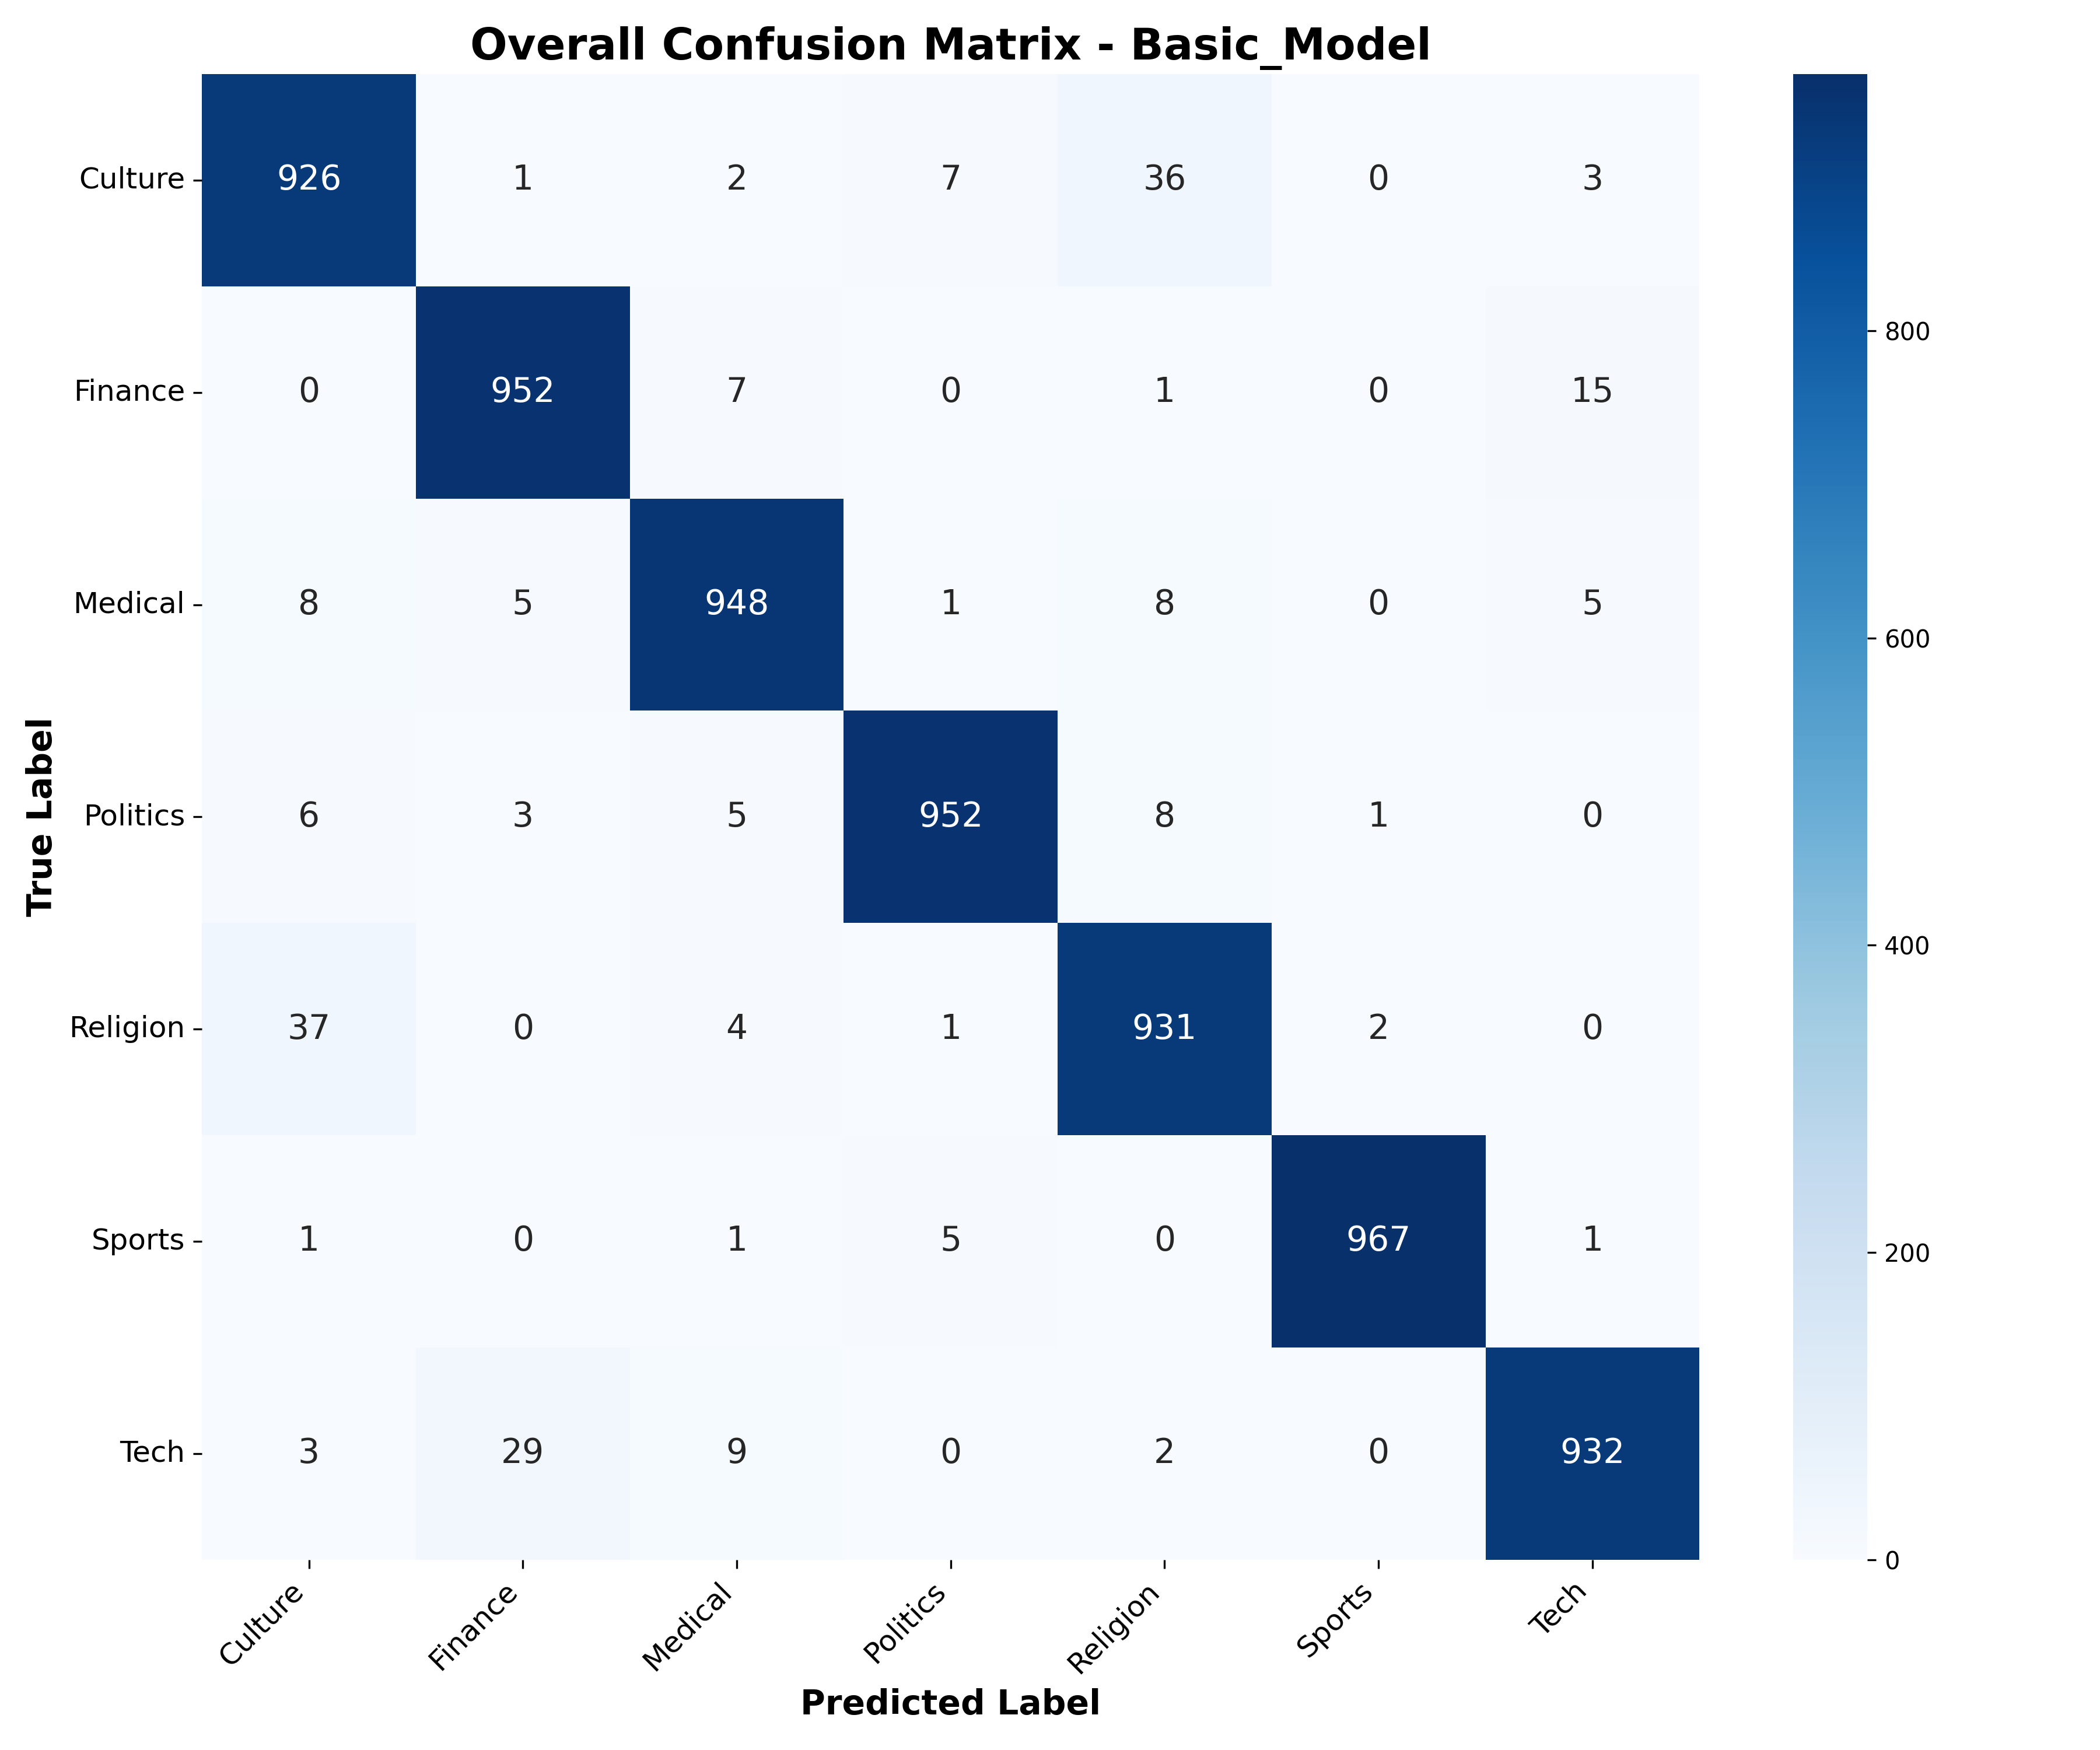
\includegraphics[width=0.9\textwidth]{overall_confusion_matrix_BM.png}
\caption{Overall confusion matrix for BERT Dense Head model across all seven news categories.}
\label{fig:cm_dense_overall}
\end{figure}

\begin{figure}[!ht]
\centering
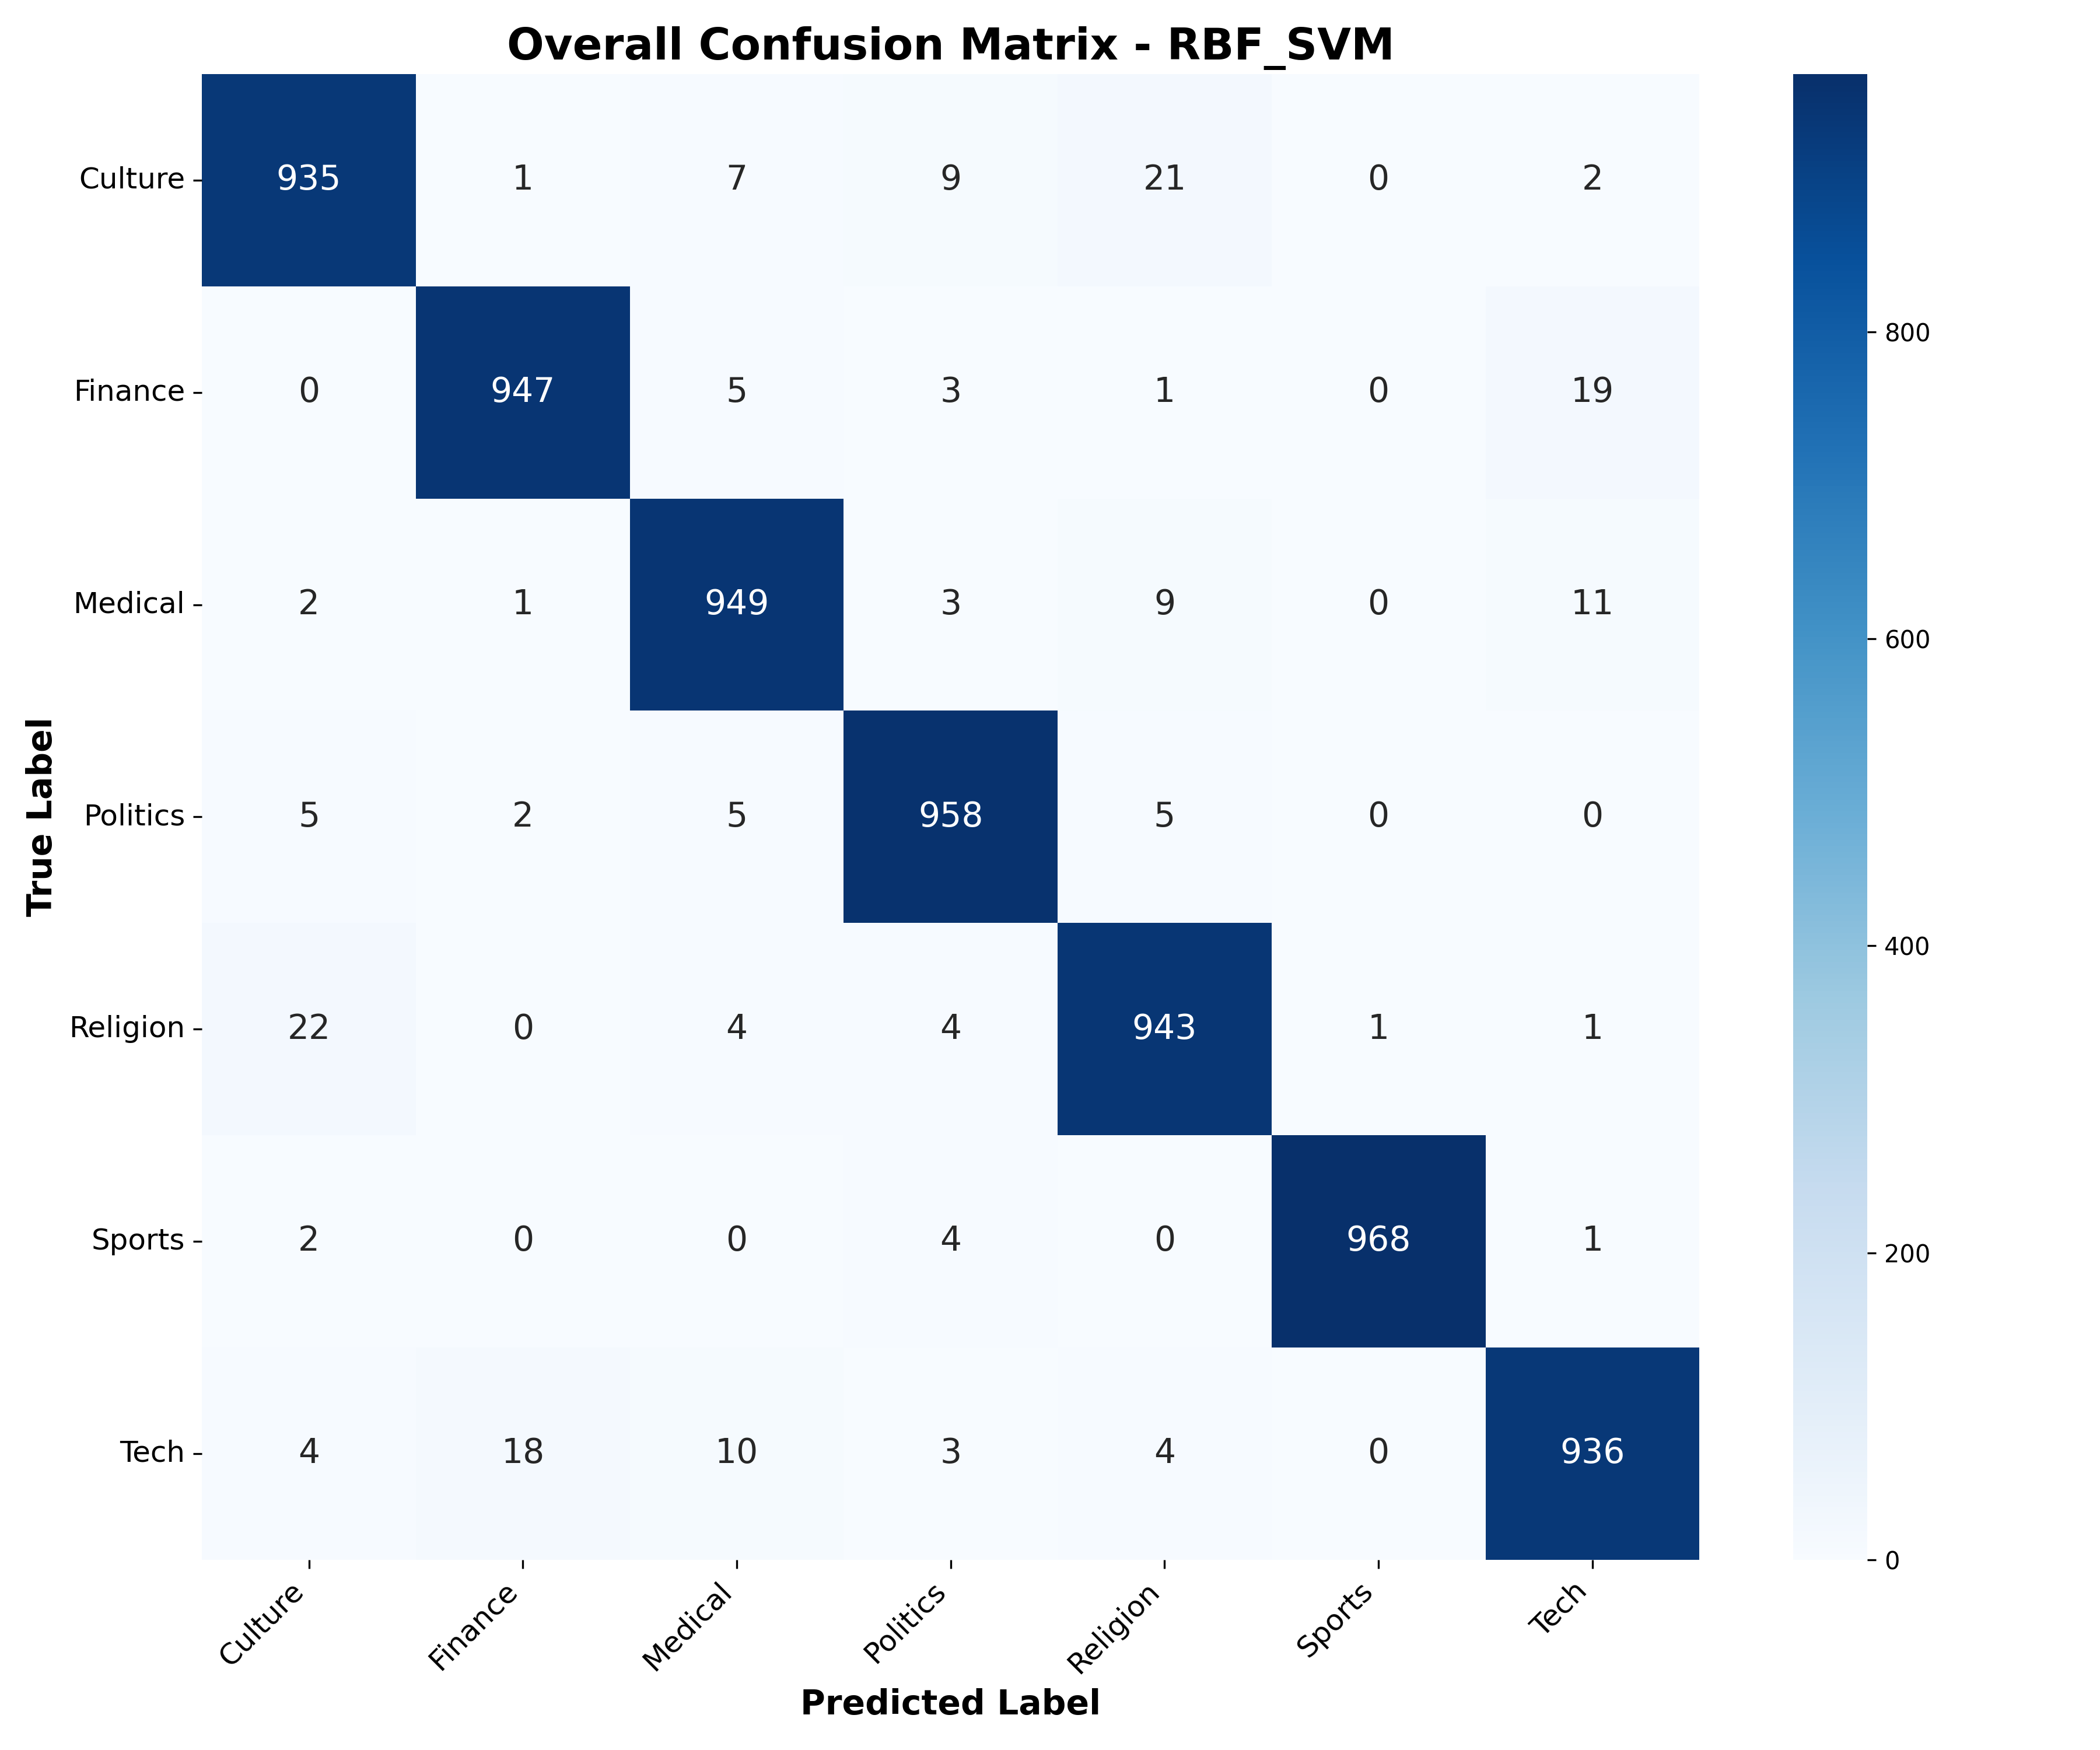
\includegraphics[width=0.9\textwidth]{overall_confusion_matrix_RBF.png}
\caption{Overall confusion matrix for BERT SVM Head model across all seven news categories.}
\label{fig:cm_svm_overall}
\end{figure}

The confusion matrices reveal several important insights. Both BERT models demonstrate exceptional performance on \textit{Sports} (967--968 correct out of 975 samples) and \textit{Finance} (947--952 correct out of 975 samples), achieving precision and recall above 0.97. In contrast, \textit{Culture} and \textit{Religion} exhibit higher confusion rates, with 37--49 misclassifications in the Dense Head and 22--40 in the SVM Head. This pattern directly relates to the challenge faced by zero-shot LLMs: categories with overlapping linguistic features and similar formal registers require domain-specific fine-tuning to distinguish effectively.

The per-class confusion matrices illuminate why general-purpose LLMs struggle with certain categories while excelling in others. \textit{Sports} maintains clear lexical boundaries (team names, player references, competition terminology) that even zero-shot models can identify reliably. However, categories like \textit{Religion}, \textit{Culture}, and \textit{Politics} share overlapping vocabulary and similar syntactic structures in Gulf Arabic journalism.

The BERT Dense Head confused 37 \textit{Religion} samples as \textit{Culture} and 36 \textit{Culture} samples as \textit{Religion}, revealing the fundamental challenge: both categories use formal MSA register, reference institutional authorities, and discuss social values. Without exposure to thousands of labeled examples distinguishing these categories, LLMs rely on surface-level heuristics that fail when contextual understanding is required. For instance, an article about a religious leader\'s comments on social issues could legitimately be classified as either \textit{Religion} or \textit{Politics} depending on framing---a nuance that fine-tuned models learn through training data patterns but zero-shot LLMs must infer from ambiguous prompts.

The confusion between \textit{Tech} and \textit{Finance} (29 misclassifications in Dense Head, 18 in SVM Head) reflects another common LLM failure mode. Technology companies in Gulf news are often discussed in economic contexts---investments, valuations, market strategies---creating lexical overlap that misleads models without domain-specific training. The SVM Head\'s improvement over Dense Head in this distinction (reducing Tech$\rightarrow$Finance errors from 29 to 18) suggests that linear decision boundaries in the embedding space can effectively separate these categories once the encoder is properly fine-tuned, whereas LLMs processing raw text struggle with this ambiguity.

Table~\ref{tab:per_class_performance} presents the detailed per-class metrics for both BERT models, computed from the confusion matrices. The \textit{Sports} category shows the most consistent results, with fine-tuned BERT models achieving near-perfect precision (0.99--1.00) and recall (0.99). The \textit{Religion} category, while still performing well in BERT models (precision 0.94--0.96, recall 0.95--0.97), shows notably more confusion with \textit{Culture} and \textit{Politics}. This explains why Claude-3.5-Haiku completely failed on \textit{Religion} (recall = 0): without fine-tuning, the model cannot distinguish the subtle contextual cues that separate religious institutional announcements from cultural or political discourse with religious references.

% \begin{table}[!ht]
% \centering
% \caption{Per-Class Performance Metrics for BERT Models}
% \label{tab:per_class_performance}
% \small
% \begin{tabular}{lcccccc}
% \hline
% \textbf{Category} & \multicolumn{3}{c}{\textbf{BERT Dense Head}} & \multicolumn{3}{c}{\textbf{BERT SVM Head}} \\
% \cline{2-4} \cline{5-7}
%  & \textbf{Precision} & \textbf{Recall} & \textbf{F1} & \textbf{Precision} & \textbf{Recall} & \textbf{F1} \\
% \hline
% Culture & 0.95 & 0.95 & 0.95 & 0.96 & 0.96 & 0.96 \\
% Finance & 0.96 & 0.98 & 0.97 & 0.98 & 0.97 & 0.97 \\
% Medical & 0.97 & 0.97 & 0.97 & 0.97 & 0.97 & 0.97 \\
% Politics & 0.97 & 0.98 & 0.97 & 0.98 & 0.98 & 0.98 \\
% Religion & 0.94 & 0.95 & 0.95 & 0.96 & 0.97 & 0.96 \\
% Sports & 0.99 & 0.99 & 0.99 & 1.00 & 0.99 & 1.00 \\
% Tech & 0.97 & 0.96 & 0.96 & 0.96 & 0.96 & 0.96 \\
% \hline
% \end{tabular}
% \end{table}
\begin{table}[!ht]
\centering
\caption{Per-Class Performance Metrics for BERT Models}
\label{tab:per_class_performance}
\small
\begin{tabular}{lccccccc}
\hline
\textbf{Category} & \multicolumn{3}{c}{\textbf{BERT Dense Head}} & \multicolumn{3}{c}{\textbf{BERT SVM Head}} \\
% \cline{2-4}\cline{5-7}
 & \textbf{Precision} & \textbf{Recall} & \textbf{F1} & \textbf{Precision} & \textbf{Recall} & \textbf{F1} \\
\hline
Culture & 0.95 & 0.95 & 0.95 & 0.96 & 0.96 & 0.96 \\
Finance & 0.96 & 0.98 & 0.97 & 0.98 & 0.97 & 0.97 \\
Medical & 0.97 & 0.97 & 0.97 & 0.97 & 0.97 & 0.97 \\
Politics & 0.97 & 0.98 & 0.97 & 0.98 & 0.98 & 0.98 \\
Religion & 0.94 & 0.95 & 0.95 & 0.96 & 0.97 & 0.96 \\
Sports & 0.99 & 0.99 & 0.99 & 1.00 & 0.99 & 1.00 \\
Tech & 0.97 & 0.96 & 0.96 & 0.96 & 0.96 & 0.96 \\
\hline
\end{tabular}
\end{table}

\subsection{Training and Inference Efficiency}
Figures~\ref{fig:train_time} and~\ref{fig:test_time} compare the supervised models. The BERT--SVM head trained in 4.38 seconds, 58.4\% faster than the Dense Head (10.54 seconds). However, inference was slightly faster for the Dense Head, making it more suitable for latency-sensitive deployment. Both models produced sub-second inference times, validating their feasibility for real-time tasks. Timing data for zero-shot LLMs were excluded, as latency was dominated by provider-side variability.

\begin{figure}[H]
\centering
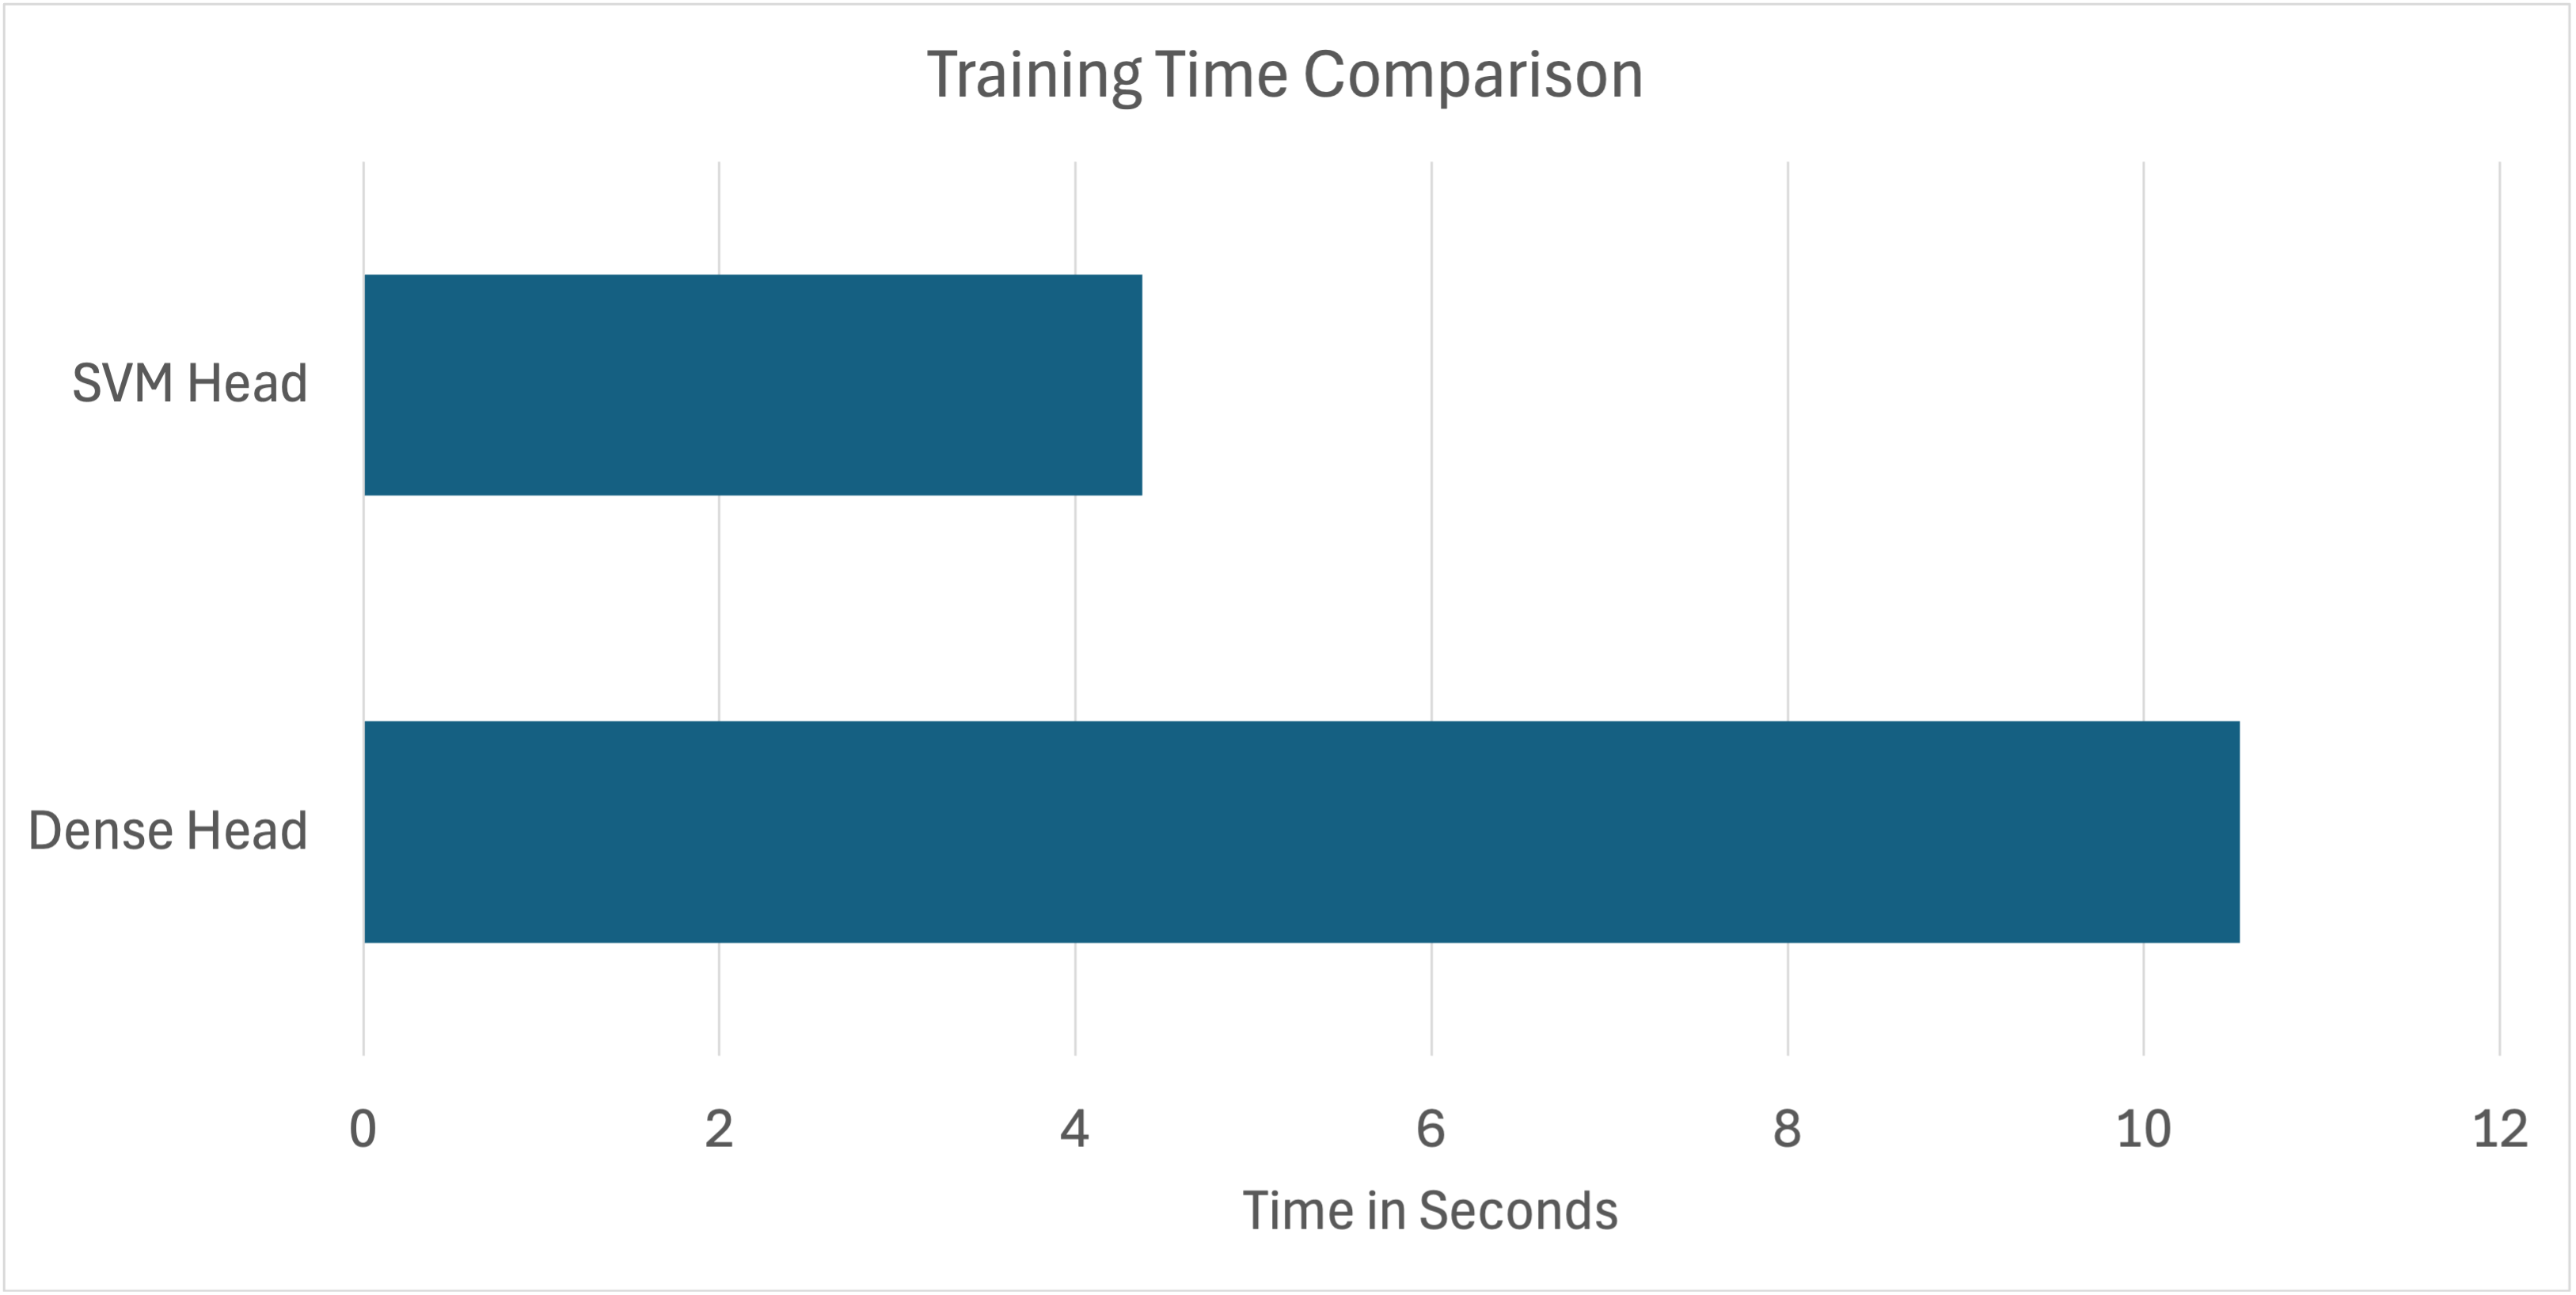
\includegraphics[width=0.9\textwidth]{Train_time.png}
\caption{Training time comparison between BERT Dense Head and BERT SVM Head models.}
\label{fig:train_time}
\end{figure}

\begin{figure}[H]
\centering
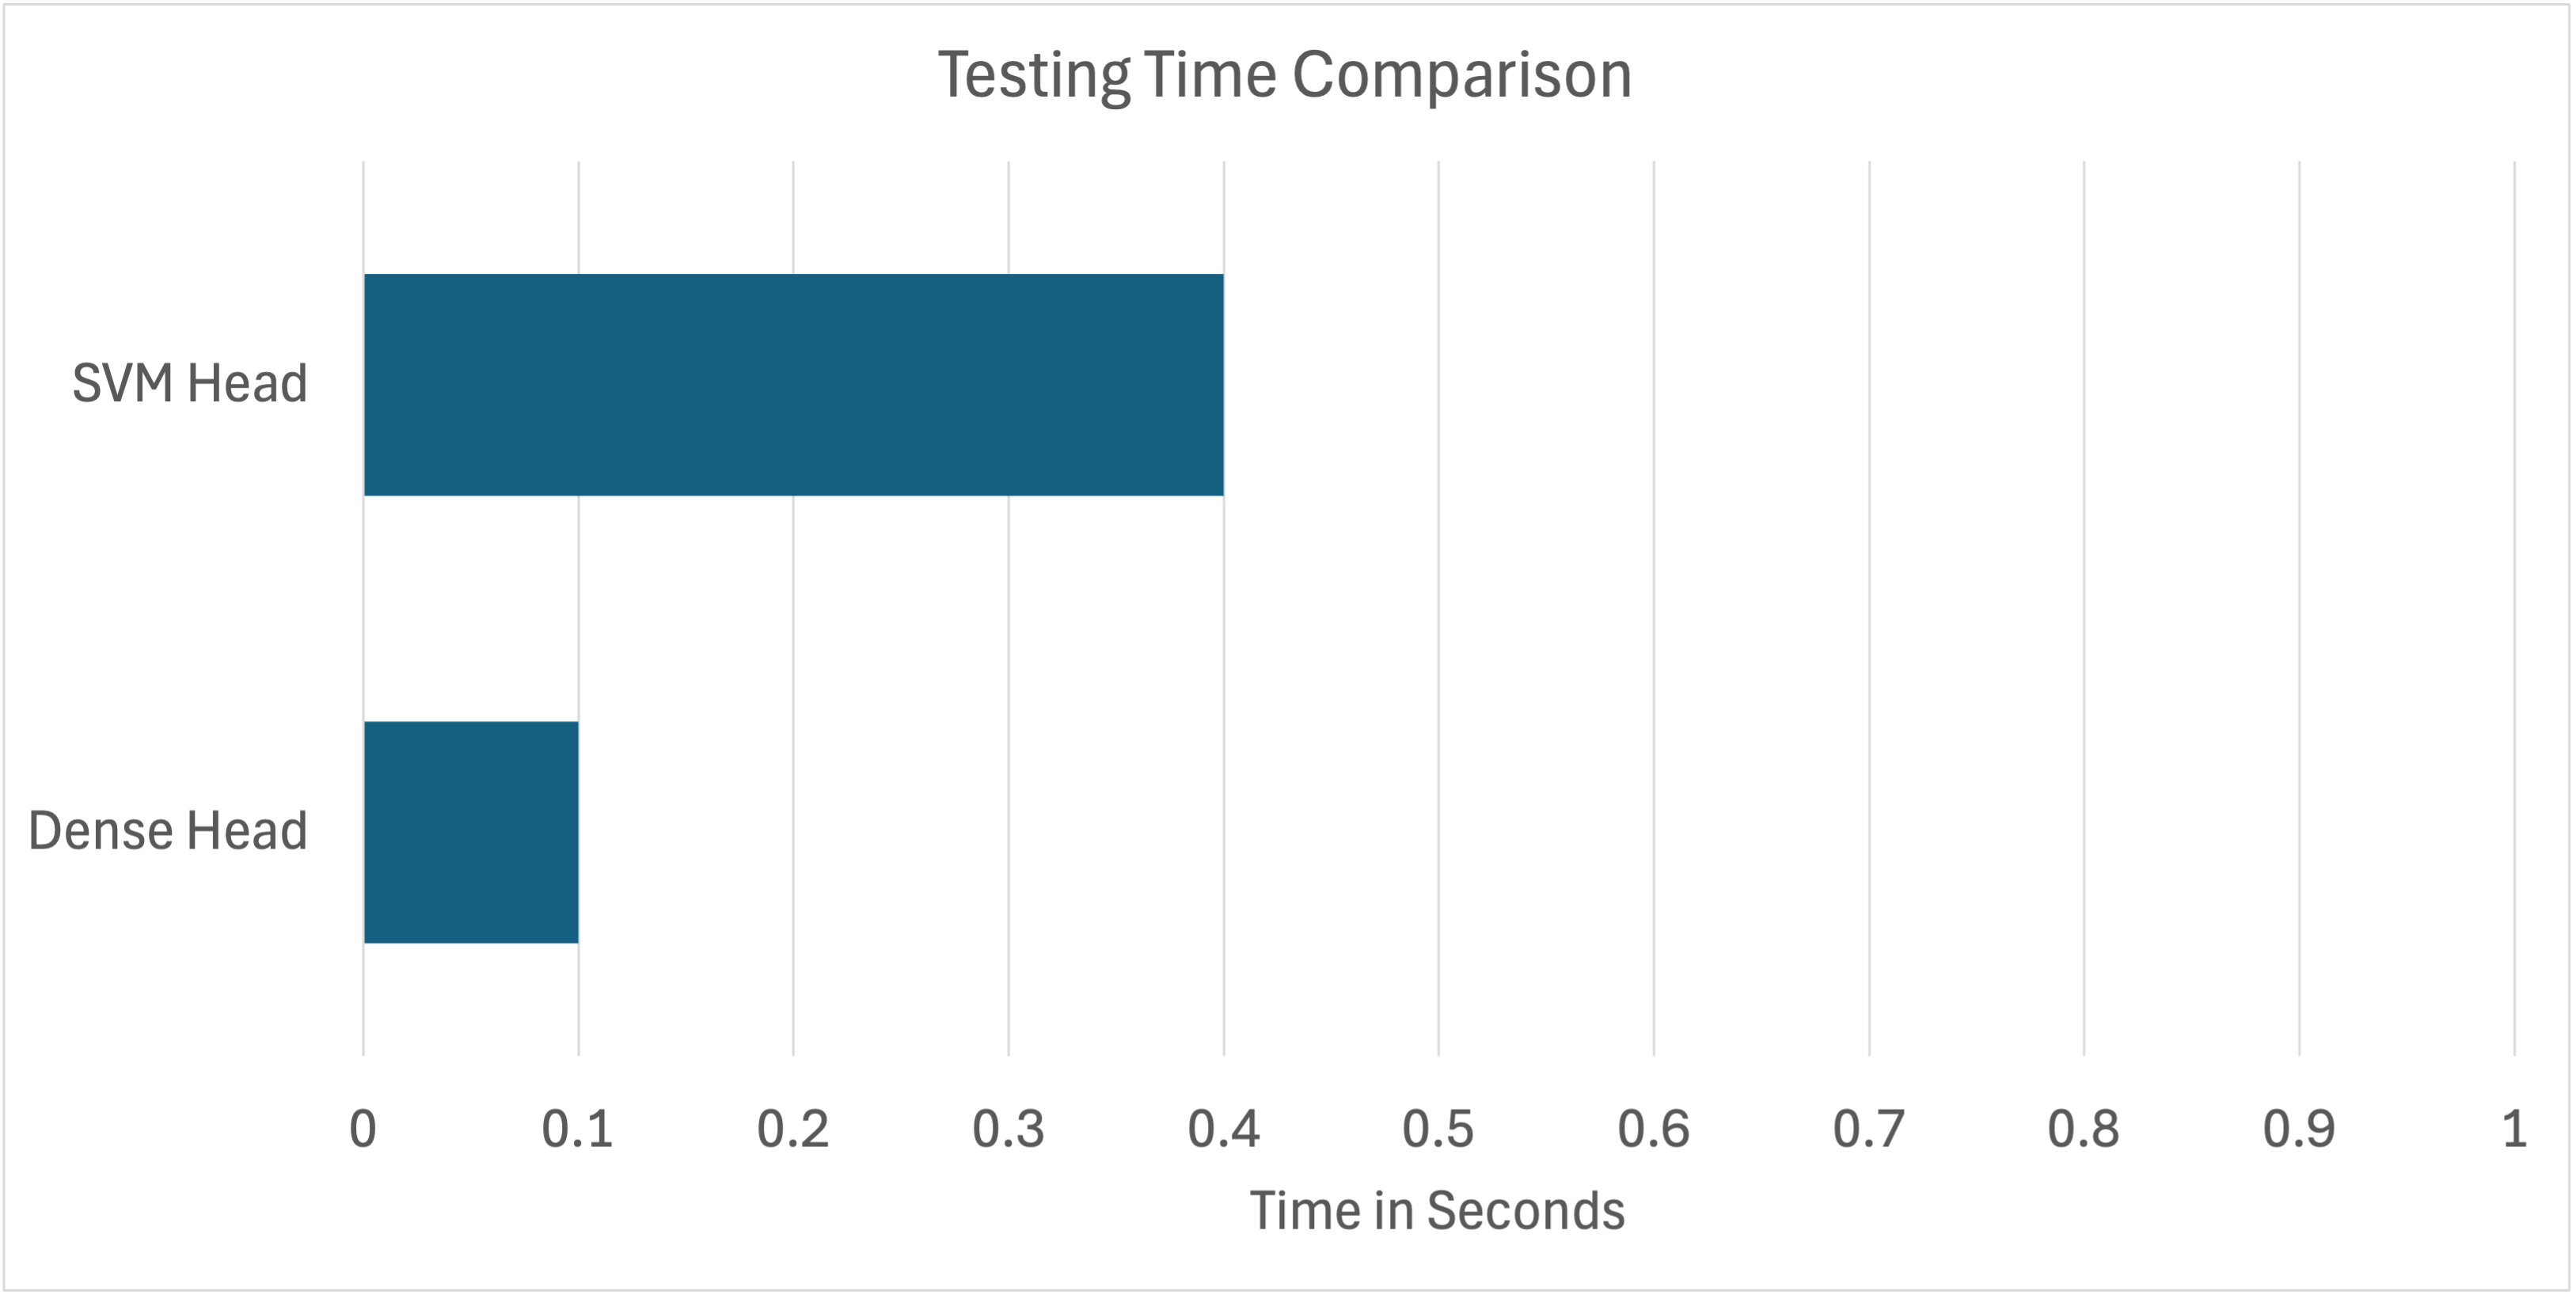
\includegraphics[width=0.9\textwidth]{Test_time.png}
\caption{Inference time comparison between BERT Dense Head and BERT SVM Head models.}
\label{fig:test_time}
\end{figure}

\subsection{Qualitative Error Analysis}

Despite overall high performance, misclassifications provide insight into model limitations. Table~\ref{tab:model-evaluation} shows examples where the BERT Dense Head failed. Financial news with embedded numeric details was sometimes mislabeled as \textit{Sports}, likely due to superficial lexical overlap. Similarly, medical-sector content was mislabeled as \textit{Religion}, showing challenges in distinguishing domain-specific entities when contextual cues are weak.

\begin{table}[h!]
    \centering
    \caption{Representative Misclassifications — BERT Dense Head}
    \label{tab:model-evaluation}
    \begin{tabularx}{\textwidth}{>{\raggedleft\arraybackslash}X c c c}
        \toprule
        \textbf{Text} & \textbf{Model Output} & \textbf{Original Output} & \textbf{Result} \\
        \midrule
        \RTL{دبي "الخليج" : أعلنت شركة "غلفا للمياه المعدنية" أنها حققت أرباحاً بلغت مليون درهم في 2015 مقارنة مع 6.4 مليون درهم في 2014، بعد خصم أعباء حقوق حكومة عجمان البالغة مليوني درهم، وتراجعت المبيعات إلى 7 ملايين كرتونة في 2015 مقابل 7.9 مليون كرتونة في 2014.} &
        Sports & Finance & miss \\
        \addlinespace
        \RTL{دبي: "الخليج" استقبل خلف أحمد الحبتور، مؤسس ورئيس مجلس إدارة مجموعة الحبتور، الدكتور ستيفن فيكتور، الرئيس التنفيذي والمدير الطبي لدى "ريجين مديكال" في دبي.} &
        Religion & Medical & miss \\
        \bottomrule
    \end{tabularx}
\end{table}

The SVM-based model produced different error patterns (Table~\ref{tab:model-svm-evaluation}). It often mislabeled \textit{Technology} news as \textit{Finance}, suggesting an over-reliance on economic keywords. This points to a sensitivity to surface-level tokens without capturing deeper semantic relationships.

\begin{table}[h!]
    \centering
    \caption{Representative Misclassifications — BERT SVM Head}
    \label{tab:model-svm-evaluation}
    \begin{tabularx}{\textwidth}{>{\raggedleft\arraybackslash}X c c c}
        \toprule
        \textbf{Text} & \textbf{Model Output} & \textbf{Original Output} & \textbf{Result} \\
        \midrule
        \RTL{دبي: محمد إبراهيم أطلقت وزارة التربية والتعليم خلال مشاركتها في "أسبوع جيتكس للتقنية" خدمتين جديدتين تضافان إلى خدماتها الذكية الأخرى.} &
        Finance & Tech & miss \\
        \addlinespace
        \RTL{دبي: "الخليج" أعلنت شركة "إل جي" أنها ستوفر أحدث الحلول التفاعلية الرقمية في دبي باركس آند ريزورتس، أكبر منتجع سياحي وترفيهي في المنطقة.} &
        Finance & Tech & miss \\
        \bottomrule
    \end{tabularx}
\end{table}


To provide a comprehensive understanding of model behavior, this section presents systematic qualitative analysis organized into three categories: (1) examples where all models correctly classify the text, (2) instances where the proposed BERT models succeed while zero-shot LLMs fail, and (3) cases where LLMs correctly predict the label while BERT models err. This analysis reveals the complementary strengths and distinct failure modes of supervised and zero-shot approaches.

\subsubsection{Correctly Classified Examples}

Table~\ref{tab:correct-examples} presents representative examples where both BERT architectures and all zero-shot LLMs achieved correct classifications. These examples illustrate the characteristics of unambiguous news articles that models handle reliably.

\begin{table}[h!]
    \centering
    \caption{Representative Examples Correctly Classified by All Models}
    \label{tab:correct-examples}
    \small
    \begin{tabularx}{\textwidth}{>{\raggedleft\arraybackslash}p{0.55\textwidth} c c}
        \toprule
        \textbf{Text} & \textbf{Category} & \textbf{All Models} \\
        \midrule
        \RTL{انضم ساندرو فاغنر مهاجم فريق دارمشتاد لفريق هوفنهايم الألماني بعقد يمتد حتى عام 2019. وأحرز فاغنر 14 هدفاً ببطولة الدوري الموسم الماضي ليصبح ثاني لاعب ألماني أكثر تسجيلاً للأهداف في البطولة خلف توماس مولر نجم بايرن ميونيخ الذي سجل 20 هدفاً.} &
        Sports & \checkmark \\
        \addlinespace
        \RTL{أكدت مجموعة الدراسات إتش سي أن صكوك شركة الدار العقارية والتي تستحق عام 2014 لم تتأثر بخفض موديز لتقييم الشركة، بل على العكس، قفز سعر الصك من 103،5 إلى 106،5 دولار في الوقت الذي لم تتغير فيه نسبة العائد، وثبتت عند 9،75\%.} &
        Finance & \checkmark \\
        \addlinespace
        \RTL{نفذت إدارة مركز الطب الوقائي في الذيد عدداً من الفعاليات المتنوعة، التي هدفت إلى سعادة الموظفين من خلال أهدافها وبرامجها، التي تعد ركناً أساسياً من أركان سمعتها الطيبة ودورها الطبي.} &
        Medical & \checkmark \\
        \bottomrule
    \end{tabularx}
\end{table}

The \textit{Sports} example demonstrates clear lexical boundaries through player names, team references, and competition terminology (goals, league, season) that all models readily identify. The \textit{Finance} example contains unambiguous financial indicators (bonds, credit ratings, yields, prices) that establish clear category membership. The \textit{Medical} example references preventive medicine centers and health-related initiatives with explicit medical vocabulary. These characteristics---domain-specific terminology, clear institutional references, and unambiguous topical framing---facilitate reliable classification across all model types.

\subsubsection{BERT Correct, LLMs Incorrect}

Table~\ref{tab:bert-correct-llm-wrong} presents cases where the fine-tuned BERT model correctly classified texts that multiple zero-shot LLMs misclassified. These examples highlight the advantages of domain-specific fine-tuning.

\begin{table}[h!]
    \centering
    \caption{Examples Where BERT Succeeded and Zero-Shot LLMs Failed}
    \label{tab:bert-correct-llm-wrong}
    \small
    \begin{tabularx}{\textwidth}{>{\raggedleft\arraybackslash}p{0.32\textwidth} c c >{\raggedright\arraybackslash}p{0.28\textwidth}}
        \toprule
        \textbf{Text} & \textbf{True Label} & \textbf{BERT} & \textbf{LLM Predictions} \\
        \midrule
        \RTL{ارتفع عدد مشتركي خطوط الهاتف المتحرك لدى شركة الإمارات للاتصالات المتكاملة دو إلى أكثر من 4 ملايين مشترك حالياً، بينما ارتفع عدد الخطوط المباعة منذ انطلاق الشركة حتى الآن إلى حوالي 7 ملايين خط.} &
        Tech & Tech \checkmark & GPT: Finance \texttimes \newline Gemini: Finance \texttimes \\
        \addlinespace[1em]
        \RTL{تذهب بعض المصادر التاريخية الى أن قطز ينتمي في أصوله الى الخوارزمية، وخاله هو السلطان جلال الدين منكبرتي آخر الخوارزمشاهية، وأنه بعد ان تغيرت الحال بأسرته استرق، وتداولته أيادي التجار، الى أن صار في جملة المماليك.} &
        Religion & Religion \checkmark & GPT: Culture \texttimes \newline Gemini: Politics \texttimes \newline Claude: Politics \texttimes \newline DeepSeek: Culture \texttimes \\
        \addlinespace[1em]
        \RTL{اعتمد المدير التنفيذي لمؤسسة دبي لخدمات الإسعاف، خليفة الدراي، تشكيل مجلس الشباب بالمؤسسة، خلال اجتماع موسع مع مديري الإدارات وكبار الموظفين والمسؤولين.} &
        Medical & Medical \checkmark & GPT: Culture \texttimes \newline Gemini: Politics \texttimes \newline Claude: Politics \texttimes \newline DeepSeek: Politics \texttimes \\
        \bottomrule
    \end{tabularx}
\end{table}

The first example illustrates the \textit{Technology}--\textit{Finance} confusion pattern prevalent among LLMs. Although the article discusses a telecommunications company (du), the numerical focus on subscriber counts and sales figures triggered financial classification by GPT-4.1 and Gemini-2.0-Flash. The fine-tuned BERT model correctly identified the technological context---mobile phone lines and telecommunications services---demonstrating its learned ability to distinguish between technology companies and financial reporting.

The second example reveals the \textit{Religion}--\textit{Culture} confusion that affected all four LLMs. The historical narrative about Qutuz, a Mamluk sultan who played a crucial role in Islamic history, was misclassified as either \textit{Culture} or \textit{Politics}. While the text employs historical narrative style that superficially resembles cultural content, it discusses Islamic historical figures in a religious-historical context. The fine-tuned model learned through exposure to labeled training data that such historical Islamic narratives belong to the \textit{Religion} category in Gulf Arabic journalism conventions.

The third example demonstrates how institutional announcements can mislead zero-shot LLMs. Despite explicit references to Dubai Ambulance Services and medical context, all LLMs classified this as either \textit{Politics} or \textit{Culture}, likely triggered by administrative terminology (board formation, executive meetings). The BERT model correctly recognized the medical institutional context.

\subsubsection{LLMs Correct, BERT Incorrect}

Table~\ref{tab:llm-correct-bert-wrong} presents contrasting cases where zero-shot LLMs correctly classified texts that the BERT model misclassified, revealing limitations of the supervised approach.

\begin{table}[h!]
    \centering
    \caption{Examples Where Zero-Shot LLMs Succeeded and BERT Failed}
    \label{tab:llm-correct-bert-wrong}
    \small
    \begin{tabularx}{\textwidth}{>{\raggedleft\arraybackslash}p{0.38\textwidth} c c >{\raggedright\arraybackslash}p{0.28\textwidth}}
        \toprule
        \textbf{Text} & \textbf{True Label} & \textbf{BERT} & \textbf{LLM Predictions} \\
        \midrule
        \RTL{قضت محكمة عمانية بالسجن ثلاث سنوات والغرامة 76 ألفاً و804 ريالات و8 بيسات على ضابط شرطة برتبة عميد، حيث أدانته المحكمة الابتدائية بمسقط بجنحتي الرشوة عن مشروع تحصيل رسوم دخول المنافذ البرية واختلاس مخصصات.} &
        Politics & Finance \texttimes & GPT: Politics \checkmark \newline Gemini: Politics \checkmark \newline Claude: Politics \checkmark \newline DeepSeek: Politics \checkmark \\
        \addlinespace[1em]
        \RTL{دبي ``الخليج'': استضاف ``مجلس الإمارات للأبنية الخضراء''، أمس، بالتعاون مع ``مجلس الأعمال الفرنسي'' بدبي فعالية خاصة حول أحدث الابتكارات الخضراء. وشارك في الفعالية ممثلون عن أكثر من 20 هيئة ومؤسسة.} &
        Tech & Medical \texttimes & Gemini: Tech \checkmark \newline Claude: Tech \checkmark \newline DeepSeek: Tech \checkmark \\
        \addlinespace[1em]
        \RTL{تستقطب قناة القصباء في الشارقة يومياً عشرات بل مئات الأسر العربية وغير العربية من مختلف الجاليات المقيمة في الامارات، وتأتي هذه الأسر مع أطفالها إلى ساحات ومرافق القناة نظراً لطبيعة المكان المفتوحة.} &
        Culture & Religion \texttimes & GPT: Culture \checkmark \newline Gemini: Culture \checkmark \newline Claude: Culture \checkmark \newline DeepSeek: Culture \checkmark \\
        \bottomrule
    \end{tabularx}
\end{table}

The first example demonstrates BERT's susceptibility to surface-level lexical cues. The article about a court case involving bribery and embezzlement charges against a police officer was misclassified as \textit{Finance} due to monetary figures (fines, amounts) and financial terminology. All zero-shot LLMs correctly identified the political/legal nature of the content through broader contextual understanding of court proceedings and governmental corruption cases.

The second example shows how BERT can be confused by institutional overlap. The Emirates Green Building Council event about green innovations was misclassified as \textit{Medical}, possibly due to associations between ``green'' terminology and health-related contexts in the training data. The LLMs' broader world knowledge allowed them to correctly associate green building technology with the \textit{Technology} category.

The third example reveals the \textit{Culture}--\textit{Religion} confusion in reverse. BERT misclassified a cultural article about Al Qasba Canal in Sharjah as \textit{Religion}, while all LLMs correctly identified the cultural/leisure content. This suggests that certain cultural venue descriptions may share linguistic patterns with religious site descriptions in the training data.

\subsubsection{Model-Specific Error Patterns}

Analysis of the 1,000-sample test set reveals systematic error patterns for each model architecture. Table~\ref{tab:error-summary} summarizes the key confusion patterns observed.

\begin{table}[h!]
    \centering
    \caption{Summary of Model-Specific Error Patterns}
    \label{tab:error-summary}
    \small
    \begin{tabular}{lll}
        \toprule
        \textbf{Model} & \textbf{Primary Confusion} & \textbf{Likely Cause} \\
        \midrule
        BERT Dense Head & Finance $\leftrightarrow$ Tech & Numerical/financial terms in tech contexts \\
        & Religion $\leftrightarrow$ Culture & Shared formal MSA register \\
        \addlinespace
        GPT-4.1 & Tech $\rightarrow$ Finance & Economic framing of technology news \\
        & Religion $\rightarrow$ Culture & Historical/narrative style overlap \\
        \addlinespace
        Gemini-2.0-Flash & Tech $\rightarrow$ Finance & Business context dominance \\
        & Religion $\rightarrow$ Culture/Politics & Institutional announcement patterns \\
        \addlinespace
        Claude-3.5-Haiku & Religion $\rightarrow$ Culture (59\%) & Fundamental category boundary issues \\
        & Religion $\rightarrow$ Politics (28\%) & Religious-political discourse overlap \\
        \addlinespace
        DeepSeek V3 & Tech $\rightarrow$ Finance & Similar to GPT-4.1 patterns \\
        & Religion $\rightarrow$ Culture & Similar to GPT-4.1 patterns \\
        \bottomrule
    \end{tabular}
\end{table}

Claude-3.5-Haiku exhibited the most severe category confusion, with 32 out of 135 Religion samples (24\%) misclassified, primarily as \textit{Culture} (59\%) or \textit{Politics} (28\%). This systematic failure suggests fundamental difficulties in distinguishing Gulf Arabic religious discourse from related cultural and political content without domain-specific training.

\subsubsection{Implications for Model Selection}

These qualitative findings yield practical recommendations for Arabic news classification deployment:

\begin{enumerate}
    \item \textbf{High-stakes applications}: Fine-tuned BERT models provide more consistent performance across all categories, particularly for Religion/Culture disambiguation where LLMs systematically struggle.
    
    \item \textbf{Technology/Finance contexts}: Consider ensemble approaches or post-hoc verification when articles contain both technological content and financial metrics, as both model families exhibit confusion in this domain.
    
    \item \textbf{Resource-constrained scenarios}: Among zero-shot LLMs, GPT-4.1 and DeepSeek V3 offer the best balance of performance and accessibility, while Claude-3.5-Haiku should be avoided for Arabic classification tasks without further prompt optimization.
    
    \item \textbf{Edge cases}: Articles with institutional announcements, historical narratives, or mixed domain terminology benefit from fine-tuned models that have learned corpus-specific classification conventions.
\end{enumerate}

These qualitative insights reinforce the quantitative findings: domain-specific fine-tuning enhances robustness, but different model heads exhibit distinct error profiles. Dense heads better capture semantic nuance, while SVM heads emphasize token-level features, leading to divergent failure cases.

%%%%%%%%%%%%%%%%





\subsection{Linguistic and Contextual Challenges for LLMs}

To strengthen the analysis, we examined the linguistic and contextual challenges faced by zero-shot LLMs in Arabic news classification, which help explain the performance gap compared to fine-tuned supervised approaches.

\subsubsection{Morphological Complexity and Tokenization}

Arabic\'s rich morphological system presents unique challenges for general-purpose LLMs. Words in Arabic are formed through complex patterns of roots and affixes, with prefixes and suffixes that can encode grammatical information such as tense, gender, number, and case. For instance, a single Arabic word can contain a conjunction, future tense marker, verb root, plural masculine suffix, and object pronoun---all in a single token. General-purpose LLMs trained primarily on English and other European languages may struggle with such dense morphological encoding, leading to suboptimal semantic understanding.

In contrast, CAMeLBERT was pre-trained on 167 GB of Arabic text using domain-adaptive tokenization strategies that better capture morphological boundaries. The fine-tuning process further specializes these representations for news categorization, allowing the model to distinguish subtle morphological patterns that signal topical boundaries. For example, technical terminology in \textit{Technology} articles often follows specific derivational patterns that fine-tuned models learn to associate with the correct category.

\subsubsection{Diglossia and Register Variation}

Arabic exists in a state of diglossia, with Modern Standard Arabic (MSA) used in formal writing and various dialects in spoken communication. News articles predominantly use MSA, but they may incorporate dialectal expressions, loanwords, or code-switching, particularly in quotes or informal sections. Zero-shot LLMs, lacking exposure to the specific stylistic conventions of Gulf Arabic news sources, may misinterpret these register shifts as topical indicators rather than stylistic choices.

The misclassification of medical content as \textit{Religion} (Table~\ref{tab:model-evaluation}) exemplifies this challenge. Both domains share formal register and may use similar syntactic structures for institutional announcements. Without fine-tuning on domain-specific examples, LLMs may over-weight superficial lexical similarities (e.g., honorific titles, formal verb forms) at the expense of semantic content. Fine-tuned models, having seen numerous examples from each category, develop robust feature representations that distinguish genuine religious content from other formal discourse.

\subsubsection{Named Entity Ambiguity and Cultural Context}

Arabic news articles frequently reference named entities---organizations, locations, public figures---whose categorization depends heavily on cultural and contextual knowledge. For example, Al-Hilal could refer to a prominent football club (\textit{Sports}) or the Red Crescent humanitarian organization (\textit{Politics or Society}). Similarly, Al-Nassr is both a sports club and a common term meaning victory used across domains.

Zero-shot LLMs, despite their broad knowledge, may lack the fine-grained understanding of Gulf region entities and their primary associations within this specific news corpus. The complete failure of Claude-3.5-Haiku on the \textit{Religion} category (0\% recall) suggests systematic misunderstanding of how religious topics are framed in Gulf Arabic journalism. This contrasts sharply with fine-tuned models, which learn corpus-specific entity-category associations during training. The supervised learning process effectively builds a domain-specific knowledge graph that captures which entities and phrases reliably predict each news category.

\subsubsection{Prompt Engineering Limitations}

The performance of zero-shot LLMs is highly sensitive to prompt design, yet optimal prompts for Arabic classification may differ significantly from English best practices due to structural and pragmatic differences between the languages. Arabic\'s VSO (Verb-Subject-Object) word order flexibility and optional case marking create ambiguities that English prompts may not adequately address. Furthermore, culturally appropriate framing of classification instructions requires understanding how category boundaries are conceptualized in Arabic journalism---for instance, where the line between \textit{Politics} and \textit{Religion} falls in coverage of religious authorities making policy statements.

Without extensive prompt optimization for each LLM and careful validation on Arabic-specific test cases, zero-shot performance remains inconsistent. The 18-percentage-point gap between GPT-4.1 (93\%) and Claude-3.5-Haiku (75\%) suggests that model architecture, training data composition, and inference-time prompt processing all significantly impact Arabic text understanding. Fine-tuned models bypass these challenges entirely, as the classification head learns optimal decision boundaries directly from labeled examples without relying on natural language instructions.

\subsubsection{Advantages of Supervised Fine-Tuning}

The consistent 97\% accuracy achieved by both BERT-based architectures demonstrates the effectiveness of supervised fine-tuning in overcoming the above challenges. Several mechanisms contribute to this success:

\begin{itemize}
    \item \textbf{Task-specific feature learning}: Fine-tuning adjusts the entire model to emphasize features relevant to news categorization, down-weighting irrelevant linguistic patterns that dominate pre-training objectives.
    
    \item \textbf{Boundary refinement}: Exposure to labeled examples from all categories allows the model to learn precise decision boundaries that separate similar domains (e.g., \textit{Technology} vs. \textit{Finance} in business contexts).
    
    \item \textbf{Error correction feedback}: The backpropagation of classification errors during training directly updates model parameters to reduce confusion between frequently conflated categories, creating category-specific feature detectors.
    
    \item \textbf{Calibrated confidence}: Fine-tuned models produce well-calibrated probability distributions over categories, reflecting genuine uncertainty in ambiguous cases rather than the overconfident or poorly calibrated predictions sometimes observed in zero-shot scenarios.
\end{itemize}

The near-identical performance of Dense and SVM heads (both 97\%) further validates that the primary performance gains come from the fine-tuned BERT encoder rather than the classification architecture. This suggests that domain adaptation at the representation level---learning Arabic news-specific semantic embeddings---is the critical factor for high accuracy.

These qualitative insights reinforce the quantitative findings: while large language models demonstrate impressive general capabilities, domain-specific fine-tuning remains essential for achieving robust performance on Arabic NLP tasks. The linguistic complexity, cultural specificity, and morphological richness of Arabic create barriers that general-purpose models struggle to overcome through zero-shot inference alone, even with sophisticated prompting strategies.

\section{Discussion}
\label{discussion}

The results highlight several important insights into the relative strengths and weaknesses of domain-adapted supervised models versus general-purpose zero-shot LLMs in Arabic text classification.

First, the domain-specific supervised models---particularly the BERT-based Dense Head and SVM Head---consistently outperformed zero-shot LLMs across all evaluation metrics. The fine-tuned models captured task-specific linguistic and morphological cues in Arabic that generalist models overlooked. For instance, in the \textit{Politics} and \textit{Finance} categories, fine-tuned models effectively recognized subtle lexical markers, collocations, and syntactic structures that carry domain-specific meaning. Zero-shot LLMs, trained on broad multilingual corpora, tended to conflate semantically close but contextually distinct terms, leading to lower precision in these categories. This demonstrates the value of explicit adaptation to domain distributions where word choice and framing strongly influence meaning.

Second, the analysis reveals a clear asymmetry in the performance of zero-shot LLMs across different categories. These models performed relatively better in more objective or factual domains such as \textit{Technology} or \textit{Sports}, where class boundaries rely on surface-level lexical cues and globally shared terminology. However, they struggled in subjective or culturally sensitive categories such as \textit{Religion}, where accurate classification requires nuanced understanding of culturally embedded references and pragmatic context. Notably, Claude 3.5-Haiku failed to classify any instance in the \textit{Religion} class. This failure suggests that the model\'s training data or alignment constraints may lead to systematic avoidance or misclassification of religion-related content, possibly due to safety filters, data gaps, or alignment bias against sensitive domains. By contrast, the fine-tuned models, trained directly on representative labeled data, learned to reliably separate culturally salient linguistic patterns that general-purpose systems avoided.

Third, we observe trade-offs in computational efficiency. The SVM Head trained more quickly than the Dense Head (4.38 vs.\ 10.54 seconds), making it more suitable when rapid retraining or limited compute resources are key constraints. However, the Dense Head delivered slightly faster inference, which is advantageous for latency-sensitive applications such as interactive systems. These results show that model choice should depend on deployment requirements rather than absolute performance alone.

Beyond accuracy and efficiency, supervised models also offered predictability and control. API-based LLMs exhibit runtime variability due to external service conditions, while fine-tuned models provided stable inference times and full transparency in training and deployment. This consistency is critical in real-world pipelines where reproducibility and predictable costs are essential.

Taken together, the findings suggest several directions for future research. One promising line is domain-adaptive pretraining for LLMs on Arabic corpora, which could bridge the gap between generalization and cultural grounding. Another is exploring few-shot prompting strategies, which may enhance zero-shot models without full retraining. Finally, extending evaluation to dialectal Arabic corpora would test the robustness of both supervised and zero-shot approaches in more linguistically diverse and realistic settings. Such directions would contribute to building hybrid systems that combine the scalability of large pretrained models with the adaptability of lightweight fine-tuning.

In summary, supervised domain-adapted models remain the most effective solution for high-accuracy Arabic text classification under current conditions. However, strategically combining them with foundation models—through domain adaptation, few-shot learning, or dialectal transfer—represents a compelling future path for both research and deployment.

\section{Conclusion}
\label{conclusion}

This study benchmarked lightweight supervised models against state-of-the-art zero-shot LLMs for Arabic multi-class text classification using the balanced SANAD (AlKhaleej) dataset. Two architectures based on CAMeLBERT embeddings—a dense neural head and an SVM classifier—were compared to leading LLMs: GPT-4.1, DeepSeek V3, Gemini 2.0-Flash, and Claude 3.5-Haiku.

The fine-tuned supervised models consistently outperformed their zero-shot counterparts across all evaluation metrics. Both the Dense and SVM heads achieved 97\% accuracy, while the best-performing LLM (GPT-4.1) reached 93\%. Claude 3.5-Haiku lagged significantly, particularly in sensitive categories such as \textit{Religion}. Class-level analysis further confirmed the robustness of fine-tuned models, especially in capturing nuanced semantic distinctions.

Efficiency evaluation showed that the SVM Head trains faster, while the Dense Head offers slightly better inference speed. In contrast, zero-shot LLMs, though capable of generalization, exhibited variable latency and reduced reliability in culturally specific contexts without task adaptation.

In conclusion, domain-specific fine-tuned models remain the most reliable and efficient option for Arabic text classification in practical settings. They offer strong performance, consistent behavior, and operational flexibility. Future research should investigate hybrid approaches—such as prompt-tuning or model distillation—that combine the generalization strengths of LLMs with the efficiency and controllability of supervised architectures, particularly for deployment in low-resource or latency-sensitive environments.

% Author contribution:

% Omar—Problem formulation, Dataset formulation, Conducting experiments, and visualization.

% Ali-verification, reviewing and editing.

% Ashraf—Problem formulation, methodology, Dataset formulation, supervision, and writing.


% \bibliographystyle{elsarticle-harv} 
%\bibliographystyle{model5-names}\biboptions{authoryear}
\bibliography{references}
\end{document}

